% Solution of the problem with Russian in tikzposter: https://tex.stackexchange.com/questions/307054/use-cyrillic-characters-in-tikzposter

% we don't want ae.sty
\expandafter\def\csname ver@ae.sty\endcsname{}

\documentclass[20pt, a3paper, portrait,
blockverticalspace=5mm]{tikzposter}

% Adding logos
\makeatletter
\newcommand\insertlogoi[2][]{\def\@insertlogoi{\includegraphics[#1]{#2}}}
\newcommand\insertlogoii[2][]{\def\@insertlogoii{\includegraphics[#1]{#2}}}
\newlength\LogoSep
\setlength\LogoSep{0pt}

\insertlogoi[width=7cm]{../img/MEPhI_logo}
\insertlogoii[width=7cm]{../img/Julich_logo}

\renewcommand\maketitle[1][]{  % #1 keys
	\normalsize
	\setkeys{title}{#1}
	% Title dummy to get title height
	\node[transparent,inner sep=\TP@titleinnersep, line width=\TP@titlelinewidth, anchor=north, minimum width=\TP@visibletextwidth-2\TP@titleinnersep]
	(TP@title) at ($(0, 0.5\textheight-\TP@titletotopverticalspace)$) {\parbox{\TP@titlewidth-2\TP@titleinnersep}{\TP@maketitle}};
	\draw let \p1 = ($(TP@title.north)-(TP@title.south)$) in node {
		\setlength{\TP@titleheight}{\y1}
		\setlength{\titleheight}{\y1}
		\global\TP@titleheight=\TP@titleheight
		\global\titleheight=\titleheight
	};
	
	% Compute title position
	\setlength{\titleposleft}{-0.5\titlewidth}
	\setlength{\titleposright}{\titleposleft+\titlewidth}
	\setlength{\titlepostop}{0.5\textheight-\TP@titletotopverticalspace}
	\setlength{\titleposbottom}{\titlepostop-\titleheight}
	
	% Title style (background)
	\TP@titlestyle
	
	% Title node
	\node[inner sep=\TP@titleinnersep, line width=\TP@titlelinewidth, anchor=north, minimum width=\TP@visibletextwidth-2\TP@titleinnersep]
	at (0,0.5\textheight-\TP@titletotopverticalspace)
	(title)
	{\parbox{\TP@titlewidth-2\TP@titleinnersep}{\TP@maketitle}};
	
	\node[inner sep=0pt,anchor=west] 
	at ([xshift=-\LogoSep]title.west)
	{\@insertlogoi};
	
	\node[inner sep=0pt,anchor=east] 
	at ([xshift=\LogoSep]title.east)
	{\@insertlogoii};
	
	% Settings for blocks
	\normalsize
	\setlength{\TP@blocktop}{\titleposbottom-\TP@titletoblockverticalspace}
}
\makeatother

% language settings
\usepackage[T2A]{fontenc}
\usepackage[utf8]{inputenc}
\usepackage[russian]{babel}

% scaling russian letters
\makeatletter
\newcommand{\xEC@family}[5]{%
	\DeclareFontShape{#1}{#2}{#3}{#4}%
	{<-5.5>#50500
		<5.5-6.5>#50600
		<6.5-7.5>#50700
		<7.5-8.5>#50800
		<8.5-9.5>#50900
		<9.5-10.5>#51000
		<10.5-11.5>#51095
		<11.5-13>#51200
		<13-16>#51440
		<16-18>#51728
		<18-21>#52074
		<21-26.88>#52488
		<26-32>#52986
		<32->#53583}{}}
\DeclareFontFamily{T2A}{cmr}{}
\xEC@family{T2A}{cmr}{m}{n}{larm}
\xEC@family{T2A}{cmr}{m}{sl}{lasl}
\xEC@family{T2A}{cmr}{m}{it}{lati}
\xEC@family{T2A}{cmr}{m}{sc}{lacc}
\xEC@family{T2A}{cmr}{bx}{n}{labx}
\xEC@family{T2A}{cmr}{b}{n}{larb}
\xEC@family{T2A}{cmr}{bx}{it}{labi}
\xEC@family{T2A}{cmr}{bx}{sl}{labl}
\xEC@family{T2A}{cmr}{bx}{sc}{laxc}
\xEC@family{T2A}{cmr}{m}{ui}{laui}
\makeatother

% or wrapping long titles
\makeatletter
\def\title#1{\gdef\@title{\scalebox{\TP@titletextscale}{%
			\begin{minipage}[t]{\linewidth}
				\centering
				#1
				\par
				\vspace{0.5em}
			\end{minipage}%
}}}
\makeatother

\title{ДЕКОГЕРЕНЦИЯ СПИНА В СТРУКТУРЕ С ЗАМОРОЖЕННЫМ СПИНОМ, ЕЁ ПОДАВЛЕНИЕ И ЭФФЕКТ НА ЭДМ СТАТИСТИКУ В МЕТОДЕ FREQUENCY DOMAIN}
\author{Александр Аксентьев}
\date{\today}
\institute{НИЯУ ``МИФИ,'' Forschungszentrun J\"ulich}

\usepackage{blindtext}
\usepackage{comment}
\usepackage{url}

\usetheme{Basic}
\usecolorstyle{Russia}
\usebackgroundstyle{Empty}
\useblockstyle{Minimal}
\usetitlestyle{Default}
\colorlet{blocktitlefgcolor}{black}
\colorlet{titlefgcolor}{white}
%\colorlet{titlebgcolor}{blue!50!black!50}

\usepackage[numbers]{natbib}

\newcommand{\home}{\string~}
\newcommand{\img}{\home/REPOS/EDM/Reports/img}
\newcommand{\Artem}{\home/REPOS/COSYINF/img/Artem}
\newcommand{\multisext}{\Artem/multisext_test}
\newcommand{\compare}{\Artem/spin_vs_polarization_fit_comp}
\newcommand{\decoh}{\Artem/decoherence_frequency_dependence}

\usepackage{paralist}
\usepackage{../style/phdstyle}

\begin{document}
\maketitle
\block{Поиск ЭДМ в накопительном кольце}{
В 2008 году коллаборацией в Брукхейвенской Национальной Лаборатории (BNL, США) был предложен эксперимент по измерению ЭДМ дейтрона, основанный на использовании эффекта ``замороженного спина'' в комбинированном накопительном кольце.~\cite{BNL:Deuteron2008} Для реализации условия ``замороженности спина,'' в случае дейтрона, чья магнитная аномалия $G<0$, применяется радиальное электростатическое поле $E_r$. в рамках коллаборации JEDI Исследовательского центра ``Юлих,'' проф. Ю.В. Сеничев предложил метод измерения ЭДМ, в котором сигналом служит частота колебаний вертикальной компоненты поляризации пучка, названный Frequency Domain Method.~\cite{Senichev:FDM} Главным достоинством этого метода является отсутствие необходимости исключать паразитную компоненту частоты прецессии поляризации, связанную с Магнитным Дипольным Моментом (МДМ), возникающую из-за неточности установки оптических элементов ускорителя.
}
\begin{columns}
\column{.5}
\block{Спиновая декогеренция в экспериментах по поиску ЭДМ}{
  Одной из главных проблем экспериментов по поиску Электрического Дипольного Момента (ЭДМ) элементарных частиц методом накопительного кольца является малость времени жизни поляризации пучка, также называемого Spin Coherence Time (SCT). Величина SCT накладывает ограничения на длительность измерительного цикла, а значит возможную точность единичной оценки частоты, и длительность полного времени измерения ЭДМ.
}
\column{.5}
\block{Причины декогеренции}{
Причиной декогеренции является зависимость частоты прецессии спина частицы, определяемой уравнением Т-БМТ, от равновесной энергии частицы. Отношение частоты прецессии спина частицы к её циклотронной частоте называется спин-тюном $\nu_s = \gamma G$, где $\gamma$ есть Лоренц-фактор частицы. В соответствии с принципом автофазировки, частицы с большей длиной орбиты обладают большей равновесной энергией, а значит и большим спин тюном. Удлинение орбиты частицы происходит по двум причинам:
\begin{inparaenum}[1)]
\item бетатронное движение, и
\item начальное отклонение импульса от референсного.
\end{inparaenum}
Поэтому в пучке наблюдается дисперсия спин тюнов частиц, следствием которой является деполяризации пучка.
}
\end{columns}
\begin{columns}
\column{.5}
\block{Подавление декогеренции}{
Декогеренция спин тюнов частиц может быть подавлена с помощью применения секступольных полей. Секступоль силы $S_{sext} = \frac{1}{B\rho}\frac{\partial^2 B_y}{\partial x^2}$ ($B\rho$ магнитная жёсткость) обладает двойным эффектом на декогеренцию: во-первых, он меняет величину коэффициента сжатия орбиты $\alpha = \alpha_0 + \alpha_1\delta$ как $\Delta\aplha_{1,sext} = -S_{sext}\frac{D_0^3}{L}$, а во-вторых, напрямую изменяет длину орбиты частицы как $\bkt{\frac{\Delta L}{L}}_{sext} = \mp S_{sext}\frac{D_0}{L}\beta_{x,y}\varepsilon_{x,y}$, где $D(s) = D_0(s) + D_1(s)\delta$ функция дисперсии, $\beta_{x,y}$, $\varepsilon_{x,y}$ соответственно горизонтальная и вертикальная бета-функция и эмиттанс.

На рисунке справа, например, показаны графики зависимости спин-тюнов частиц от их начального вертикального смещения, в идеальной структуре с ``замороженным спином'' до (синяя) и после (оранжевая линия) оптимизации градиента секступоля, расположенного в максимумах $\beta_y$ (остальные секступоли в этой структуре не применяются). Видно, что после оптимизации, спин тюн практически не зависит от вертикального положения частицы в вакуумной камере.
}
\column{.5}
\block{}{
\centering
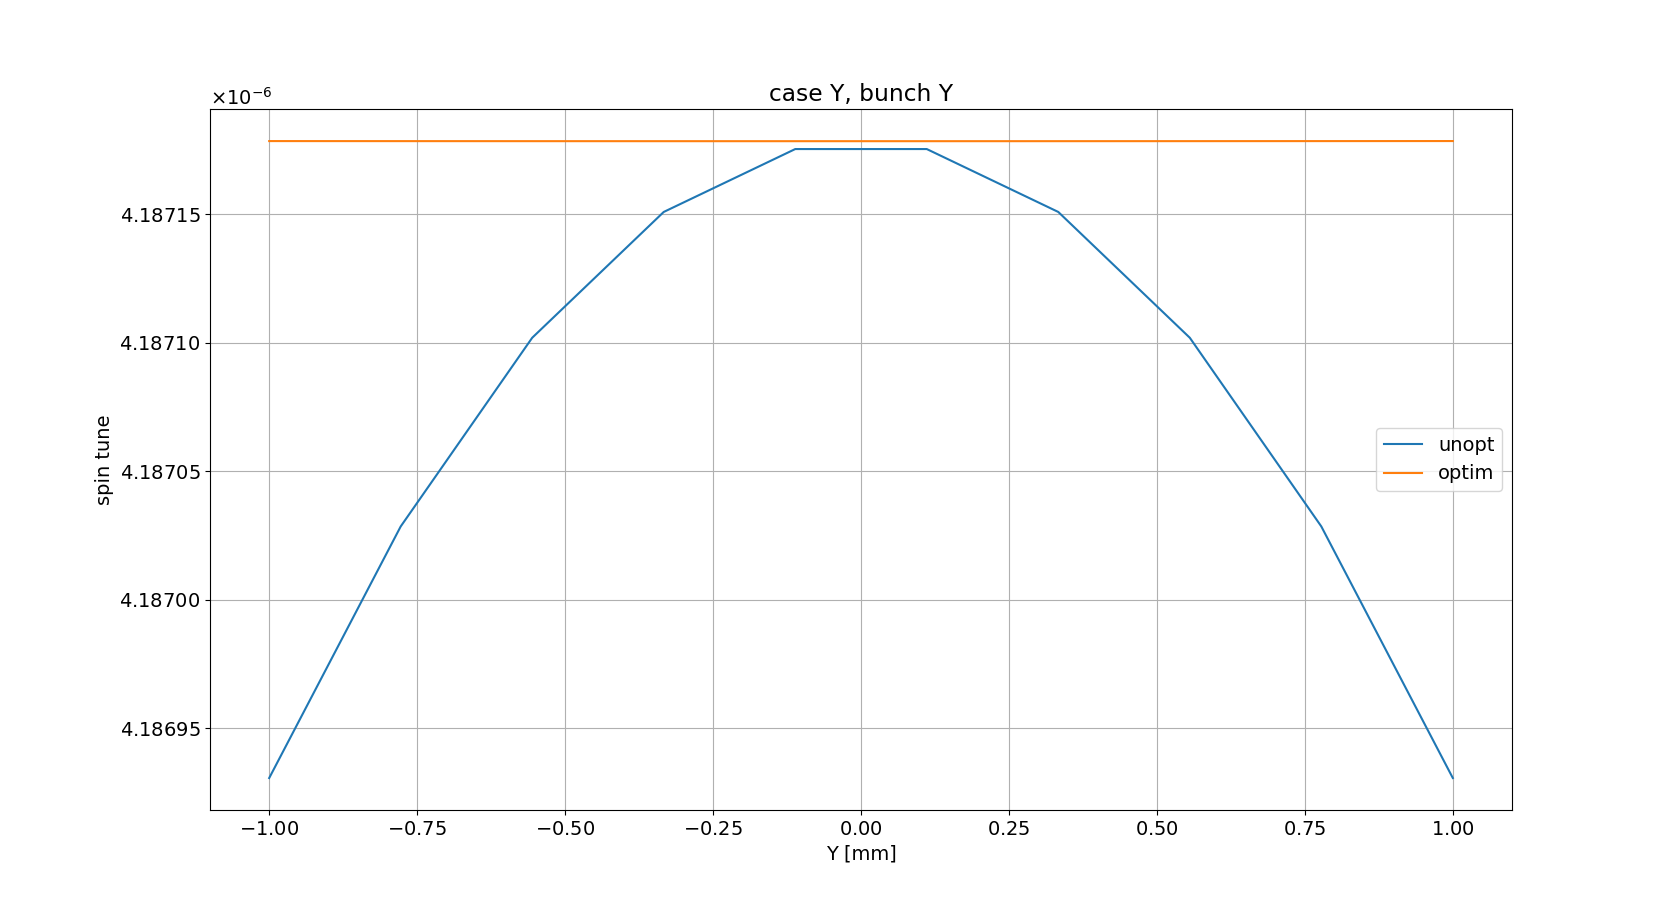
\includegraphics[width=\linewidth, trim=80 25 120 55, clip]{../SEMINAR/spin_tune_decoh_plot}
}
\end{columns}
\begin{columns}
\column{.5}
\block{Симуляция}{
Мы просимулировали спин-орбитальную динамику плоского пучка, смещённого от референсной орбиты в вертикальном направлении на $y_0 \in \bkt*{-1 mm, +1 mm}$ и распределённого в плоскости y-z как $y \sim N(0, 0.1 mm)$ в структуре с замороженным спином~\cite{Senichev:Lattices}, с E+B элементами наклонёнными вокруг оптической оси на случайные углы, взятые из распределения $\alpha\sim N(0, 5\cdot 10^{-4})$ радиан. В структуре варьировались значения градиента секступоля GSY, подавляющего декогеренцию в вертикальной плоскости, в диапазоне $\pm 5\cdot 10^{-3}$ от значения $\mathrm{GSY0} = -2.5\cdot 10^{-3}$, оптимального для идеальной структуры. Вычисленное по формуле $\vec P(n) = \frac{\sum_i \vec s_i(n)}{||\sum_i \vec s_i(n)||}$ значение поляризации пучка через оборот $n$, $\vec s_i = (s^i_X, s^i_y, s^i_z)$ спин-вектор i-ой частицы, фитировалось функцией $f(t) = a\cdot\sin(2\pi\cdot f\cdot t + \phi)$, $(a,f,\phi)$ фитируемые параметры.
}
\column{.5}
\block{}{
\begin{center}
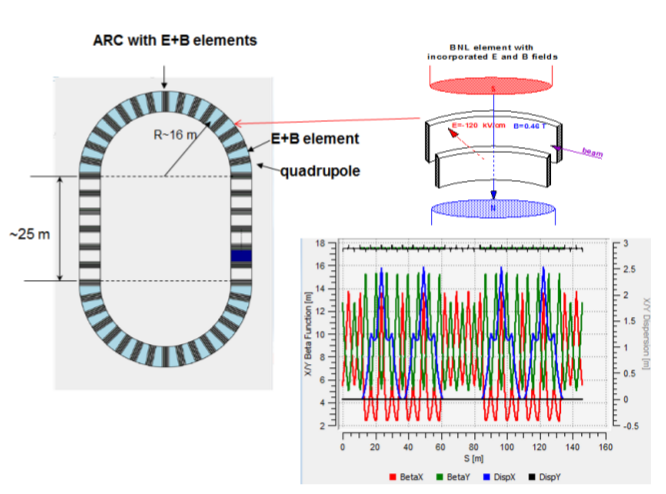
\includegraphics[width=.5\linewidth]{\img/Lattice/BNL}~
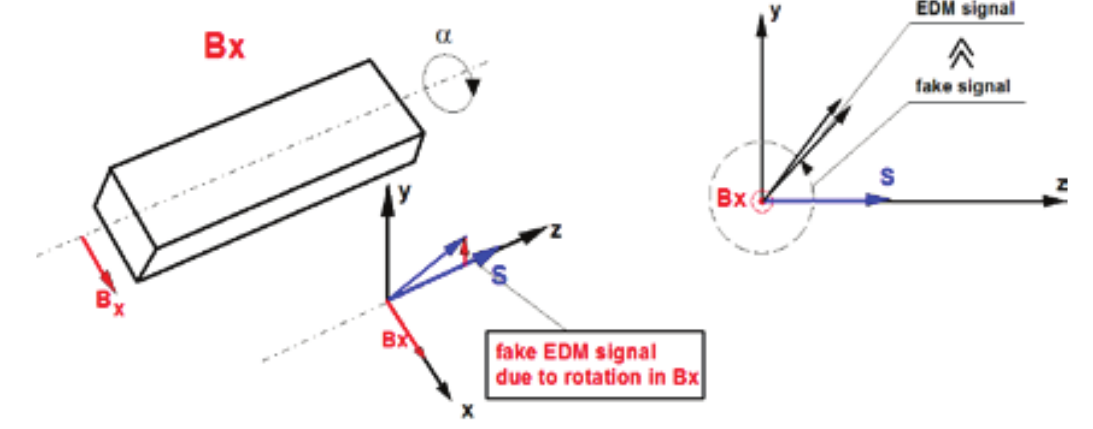
\includegraphics[width=.5\linewidth]{\img/Lattice/magnet_tilting}
\end{center}
}
\end{columns}

\block{Выводы}{
Мы обнаружили зависимость оценки частоты $\hat f(\nu_s)$ от среднего уровня   спин-тюна центроида пучка. Мы также обнаружили, что, по меньшей мере  в данной структуре, средние уровни спин-тюна и компонент оси стабильного спина связаны линейно.

\begin{center}
\includegraphics[width=.45\linewidth, trim=85 25 120 55, clip]{\decoh/freqY_vs_mean_spin_tune}~
\includegraphics[width=.45\linewidth, trim=85 25 120 60, clip]{\decoh/mean_nbar_vs_mean_spin_tune}
\end{center}
}

\block{}{
\footnotesize
\bibliographystyle{abbrv}
\bibliography{\home/REPOS/EDM/Reports/PhD/PhDRefs}
}
\end{document}
